
\section{Aprendizaje}\label{aprendizaje}
 
En el área de inteligencia artificial asociada a robótica existen variadas técnicas que permiten que un robot pueda ''aprender" a realizar alguna tarea. En este caso particular se utiliz\'o la técnica de aprendizaje por reforzamiento basado en MDP (Procesos de desici\'on Markovianas) que consiste en dar recompensas positivas o negativas dependiendo del desempeño del robot.


Segun el \cite{Mitchell} todo aprendizaje se define por la realizacion de una tarea $T$ por medio de una experiencia $E$ medido por un desempeño $D$. La tarea es aprender cual es la mejor accion a tomar dependiendo de un estado $s$ para llegar a la pelota, la experiencia es generada por TANTOS experimentos realizados y el desempeño se mide con la realizacion de la accion que genera una distancia menor a la pelota.

Se utilizó el modelo de aprendizaje Q-learning para realizar la tarea definida se presenta y describe la implementación del aprendizaje utilizado a continuación.

\subsection{Modelo Apredizaje}

Definici\'on de el modelo implementado

\subsubsection{Estado}

Un estado es definido por la posicion de la pelota, por lo tanto dada la division de las regiones de la c\'amara  se  obtienen 14 estados definidos en la siguiente imagen ~\ref{fig:estados}.

\begin{figure}[hbtp]
\centering
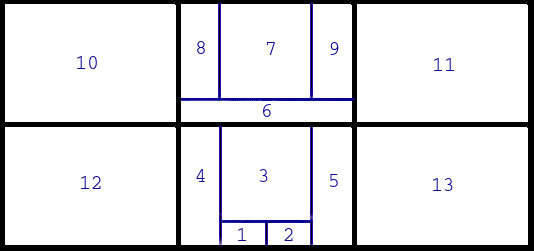
\includegraphics[scale=0.5]{imagenes/Regiones.jpg}
\caption{Estados definidos seg\'un la posici\'on de la c\'amara}
\label{fig:estados}
\end{figure}

El estado n\'umero 14 se define cuando en un barrido completo de la camara no se encuentra la pelota

\subsubsection{Acciones}

Las posibles acciones a realizar dependiendo el estado en que se encuentre son 

\begin{itemize}
\item Caminar un poco 
\item Caminar medio
\item Caminar largo
\item Girar poco derecha
\item Girar derecha
\item Girar poco izquierda
\item Girar izquierda
\end{itemize}

\subsubsection{Medida de desempeño}

La recompensa positiva o negativa se otorga dependiendo de la medida de desempeño de un estado al siguiente estado. Se entiende como un buen desempeño que dada una distancia inicial a la pelota, con una acción se llega al siguiente estado en el cual la distancia a la pelota debe ser menor que la distancia inicial, de lo contrario sera un mal desempeño y por lo tanto una recompensa negativa.

El criterio de proximidad (medida de distancias relativas) se definió en función de las regiones generadas por los movimientos de la camara con valores en el intervalo de [1 - 10] donde 1 es lo mas cercano al robot (Zona de pateo) y 10 es lo mas lejano que puede ver en un barrido de la c\'amara. Se estableci\'o el castigo como \[C(s,s') = -ds'/ 10 \] dado un estado  $ s$ a un estado $s'$ hay penalización si la distancia de $s'$ es mayor a la de $s$ entonces la distancia obtenida en $s'$ se divide entre 10 el cual es el máximo valor de distancia relativa a la pelota con ello los valores de la penalización se encuentran en el rango de [ 0 - 1 ] . Analogamente se define el premio como \[P(s,s') = 1 /ds' \] obteniendo de la misma manera un rango de valores para las recompensas positivas de [ 0 - 1 ] 

Una mejor visualizaci\'on se puede apreciar en la figura ~\ref{fig:distancias}
\begin{figure}[hbtp]
\centering
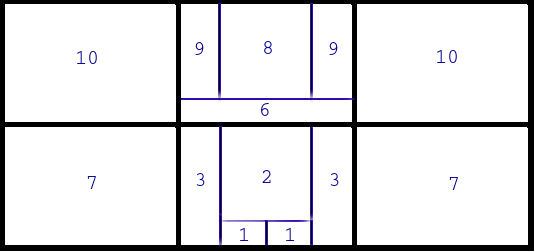
\includegraphics[scale=0.5]{imagenes/Distancias.jpg}
\caption{Distancias relativas de la pelota establecidas para otorgar la recompensa.}
\label{fig:distancias}
\end{figure}


\subsubsection{Eleci\'on de la acci\'on}


Se entiende que dado un estado se tienen 7 posibles acciones que en el entrenamiento del robot el aprende cual es mejor realizar según el estado en el cual se encuentra. Para que el aprendizaje obtenga mejores resultados se debe tener un equilibrio entre la exploración y la explotación. 

Para variar entre la explotacion y la exploracion se utiliz\'o la funcion de probabilidad definida como  \[P(a_{i} | s) = k^{Q(s,a_{i})}/ \sum_{j}k^{Q(s,a_{j})}  \] 
 
 
 
 
 